\SetKw{KwFrom}{from}
\SetKw{KwTo}{to}
\SetKwFor{KwWhile}{while}{do}{end}

\chapter{Introduction}

The modern economic development, followed by fast growth rate of the population
imposes especially significant stress for both private and public transportation
systems. This leads to an increase in the number of congestions and accidents 
on roads and has an impact on the everyday life of residents and commuters,
efficiency of resource utilization and the state of the environment. To tackle
said challenges, modern planning authorities utilize various aspects of
\textit{Intelligent Transporation Systems (ITS)}. It encompasses
state-of-the-art technologies, mainly for communication and data analysis, to
optimize and improve safety of the transportation systems.

The development of various types of sensors installed along the roads provides
new types and amounts of recorded data, the analysis of which proves to be
useful for the advancement of the modern ITS. An \textit{Inductive loop detector
(ILD)} consists of one or more coils embedded in the road pavement
\cite{Lamas.2016}. As vehicles pass above the coils, a slight change in
inductance can be observed through isolated cables that connect it to the
control cabinet \ref{fig:loop-detector}. Apart from using these signals for more
efficient traffic management, recording these registrations allows to draw
statistics on the usage level in specific time slots on road intersections where
the detectors are installed.

\begin{figure}
	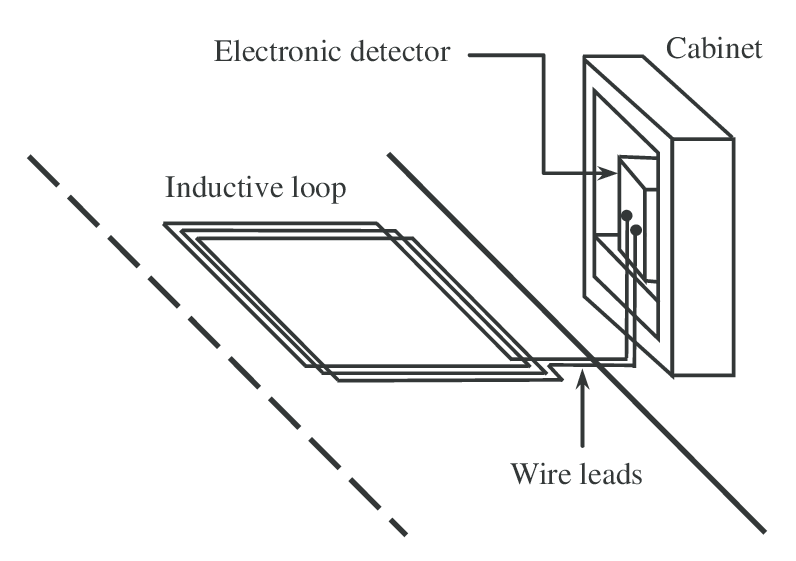
\includegraphics[width=0.5\textwidth,height=\textheight,keepaspectratio]{img/Elements-of-an-inductive-loop-detector.png}
	\centering
	\caption{Elements of an inductive loop detector. \cite{Lamas.2016}}
	\label{fig:loop-detector}
\end{figure}

One of the crucial components of ITS is short-term traffic flow prediction. It's
purpose is to estimate the amount of vehicles present of passing through a point
in the road system. We are given a data set representing the traffic density in
the city of Ingolstadt, Germany. The set is organized into 115 folders. Each
folder represents an intersection in the road network of the city of Ingolstadt
and is named after that intersection using a 4-digit code. It contains 365
\textit{csv}-files - one for each day in the year 2021. Each file is a data
table with readings from detectors as the number vehicles counted by the
detectors in 15-minute intervals. The name of a file specifies the date and
follows the format \textit{DetCount\char`_2021<month><day>.csv}. Apart from the
exact time stamps of measurements (the \textit{DATUM} column), the columns of
the tables represent the names of the detectors. Each detector is installed on a
separate lane approaching the intersection, and their names are unique within
each intersection, i.e., folder. The exact mapping between the name of a
detector within the target intersetion and the corresponding source of traffic
for it's lane is given in an additional spreadsheet called
\textit{Look Up Table (Detectors Mapping on links).xlsx}, global for the whole
data set. This file has a separate entry for each lane, including such data as
the street names, starting and ending intersection codes and names of relevant
detectors on the ending intersection. Some discrepancies between the Look-up
table and actual data files, as well as fixes for them and other issues in the
provided data set are given in Section \ref{sec:data-preparation}.

The goal of this project is to study various methods for short-term traffic
state prediction using \textit{deep learning}, select the most fitting one,
implement it if a ready realization is not available and test on the given data
described above. These methods differ from each other by considering a city
environment versus a freeway network, incorporating different types of input
data and prediction model architectures.

As part of the efforts for development and integration of ITS, researchers
usually approach the task of short-term traffic flow prediction in one of the
two ways: statistic and neural networks \cite{Karlaftis.2011}.

Early statistics-based methods are usually based on probabilistic modelling of 
data. Assuming an underlying probability distribution of traffic conditions,
they aim to capture parameters and patterns for generating the data. However,
most of them assume a linear dependency between values, which makes them less
efficient in a nonlinear setting.

\textit{Autoregressive integrated moving average (ARIMA)} \cite{Min.2011} uses
historical univariate data to analyse and forecast the trend. The popularity of
this method has made it a baseline for comparison in many research papers. To
account for more factors and extreme conditions, ARIMAX \cite{Tsirigotis.2012}
was introduced as it's multivariate extension.

\textit{Support vector regression (SVR)} \cite{Muller.1997} applies the
techniques of \textit{Supprt vector machines (SVM)} \cite{Mukherjee.1997} to
linearly separate data in a high-dimensional space after mapping to it from a 
low-dimensional space.

\textit{K-nearest neighbors(KNN)} \cite{Zhang.2013} has a very simple algorithm
that is able to derive prediction directly through data analysis without
involving complex functions. When designed with an adequate search mechanism, it
can consider both temporal and spatial parameters, as well as incorporate other 
factors.

Other examples include \textit{Kalman filtering} \cite{Guo.2014},
\textit{support vector machines (SVM)} \cite{Yang.2006}, \textit{Markov chains}
\cite{Qi.2014} and \textit{Bayesian networks} \cite{Wang.2014}.

Neural networks, on the other hand, are more flexible with input parameters
thanks to their complex architectures encompassing tens of thousands neurons.
Moreover, they are proven to handle nonlinear data much better than their more
traditional counterparts \cite{Chan.2012}. The extensive flexibility of various
architectures has allowed the researchers to not only adapt and apply neural
networks in many different domains, but experiment with different approaches to
solve each specific task. \textit{Deep Belief Network (DBN)} is a deep learning
method that relies on \textit{Restricted Boltzmann machines (RBM)}
\cite{Hinton.2006} for pre-training and was successfully applied by
\citet{Huang.2014}, showing much better results compared to shallower models.
\textit{Convolutional neural network (CNN)} \cite{Krizhevsky.2012} use filters
on neighboring inputs, making them more efficient in grid structures like
images, thus being useful for capturing spatial relationships in road networks.
\textit{Long short-term memory network (LSTM)} \cite{Graves.2013} is a special
type of a \textit{recurrent neural network (RNN)} that solves the problem of
vanishing gradients traditional for this type of models.


\chapter{Literature}

There are multiple works that aim at adapting widely used deep network
architectures for the problem of traffic state prediction. CNNs rely on
neighboring relationships, while LSTMs are good at preserving information across
long sequences of data. \citet{Yuankai.2016} combine both these models for
traffic flow prediction using a method called \textit{(CLTFP)}. As CNN filters
inputs spatially, LSTM capture short-term variation and long-term periodicity to
extract sptial-temporal features. The final prediction is then achieved with a
linear prediction layer. Being one of the earlier attempts on applying deep
learning techniques to the problem, CLTFP is claimed to show significant
improvements over it's predecessors. However, the method was tested on values
collected from 33 locations, making it wastly different from the grid structure
observed in our data.

The idea of LSTM is based on the \textit{gating} mechanism, which allows the
model to learn additional parameters used to ignore data on specific steps of
processing a recurrent sequence. This removes unnecessary operations with data
and parameters, thus solving the problem of vanishing and exploding gradients.
\textit{Gated recurrent unit (GRU)} \cite{Chung.2014} is a primary example of
executing this idea. \citet{Zhang.2018} further explore and specify this idea by
introducing a \textit{deep GRU recurrent neural network (DGRNN)}. Integrating it
into a fully-connected model allows them to discover both short and long term
correlation in data series. Unfortunately, their data format is very different
as well. While being collected from detectors placed in a grid structure in the
state of California, their features are augmented with very detailed weather
conditions. The traffic detector readings themselves are represented with
vehicle miles travelled (VMT) sampled hourly, compared to our passing vehicle
counts sampled each 15 minutes.

\citet{Liu.2019} propose an \textit{attentive traffic flow machine (ATFM)}. In
it, the first \textit{ConvLSTM} \cite{Shi.2015} unit takes input from the
original traffic flow features, as well as the memorized representations of
previous moments and uses an attention mechanism no build a weight map. The
second unit adjusts the spatial dependencies with the attentional map to
generate a spatial-temporal feature representation. For short-term prediction,
they use a customized \textit{ResNet} \cite{He.2016} for the initial feature
extraction, followed by \textit{Sequential Representation Learning} and
\textit{Periodic Representation Learning}, both of which utilize ATFM in a
recurrent manner - and finally get the prediction using a
\textit{Temporally-Varying Fusion} of their own design. Moreover, they further
extend their method for a long-term traffic prediction. However, their approach
was tested on TaxiBJ \cite{Zhang.2017} and BikeNYC \cite{Zhang.2016} data sets,
both of which contain GPS trajectories rather than passage counts.

In an attempt to leverage the best of all worlds, \citet{Hassannayebi.2021} use
a \textit{1-dimensional convolution neural network (1DCNN)} to extract traffic
flow local trend features and two types of gated RNN (LSTM and GRU) for long
temporal dependencies trend features. An attention-based \textit{dynamic optimal
weighted coefficient algorithm (DOWCA)} is then used to calculate dynamic
weights of the outputs of CNN-LSTM and CNN-GRU. The resultant \textit{combined
deep learning prediction (CDLP)} model is optimized to minimize the sum of
squared errors and shows better results than the baseline models. Unfortunately,
it has been tested on a single intersection of two roads, rather than the whole
network, which makes us question the relevance of this promising method for the 
task at hand.

Following a more traditional deep-learning based approach, \citet{Han.2020}
propose to use the combination of a feature extractor based on a deep belief 
network with a \textit{kernel extreme learning machine (KELM)} as a final
prediction model. Using this combined architecture (DBN-KELM) for the prediction
of residual noise and \textit{singular spectrum analysis (SSA)}
\cite{Leles.2017} for the trend forecast, they achieve an improved accuracy
compared to base models. On top of that, they introduce a compression method
that allows to greatly reduce the training time by applying the method to a
subset of the global data. In the original work, DBN-KELM was tested on a
freeway network of a much smaller magnitude, giving us no guarantee of success
in a city environment. However, the data here still look the most similar
compared to other listed approaches, and the method can clearly be adapted for
our purposes. Therefore, it was selected for our project. The next chapter gives
a more detailed description of all steps involved in the original work, and
Section~\ref{sec:impl-details} dives deeper into our implementation.


\chapter{Method description}

The method presented in \citet{Han.2020} is a novel deep-learning based approach
to short-term traffic state forecast. It includes an elaborate tool for time
series prediction via separation into two components, as well as a data
compression method aimed at reducing the necessary steps of the algorithm.

As an overview, the procedure starts with separating entrances (approaches) to 
intersections into groups with the highest internal degree of correlation. One
representative approach is selected from each group for further processing. 
When predictions are obtained for each selected entrance, they are being
extrapolated from each representative to it's respective group to produce a
forecast for the whole network. Applying the method for each group is possible,
however the grouping mechanism allows to decrease the number of times the
prediction techniques are applied, saving the running time.

For each entrance, the data series is being split into two components
(\textit{trend} and \textit{residual}) using the \textit{fast Fourier transform
(FFT)}. The prediction for the trend component is obtained via the
\textit{Overlap-SSA} \cite{Leles.2017}, while the residual is fed into a deep
architecture which is the main subject of the paper. The model uses a DBN for
feature extraction and a KELM for the final prediction. When the predicted
sample is obtained for both components, they are added back together to produce 
the final forecast.

The rest of the chapter describes each used technique in details and explains
the place they hold in the general approach.


\section{Expected input data format} \label{sec:expected-data}

The data as expected by all presented techniques consist of a set of time 
series, each containing integral values representing the numbers of vehicles 
that passed through a fixed point in space in equal time periods. In practice,
an individual sequence of numbers is to be taken from all detectors located on
the same \textit{entrance} to an \textit{intersection}, i.e., on all lanes
entering it. Thus, each direct \textit{connection} between two intersections
contains one or two \textit{sections} - for each direction - and each section
provides one sequence of vehicle counts collected from all detectors installed
on the relevant entrance.

Formally, if the network is represented as a directed graph $G=(N,E)$, $N$ will
represent the set of all intersections and $E=\{s_i,i=1,2,\ldots,p\}$ - all $p$
sections connecting them in various directions. Let $d$ be the number of samples
in the series. Then, for each section $s_i$, denote an individual reading from a
counter in the period $(t_{j-1},t_j)$ as $z(s_i,t_j)$. The whole traffic flow
from $t_1$ until $t_d$ for $s_i$ will be a vector
$\mathbf{q}_i=\{z(s_i,t_1),z(s_i,t_2),\ldots,z(s_i,t_d)\}$. Stacking these
vectors for all $p$ sections will produce a matrix
$\mathbf{Q}=[\mathbf{q}_1,\mathbf{q}_2,\ldots,\mathbf{q}_p],\space\mathbf{Q}
\in\mathbb{R}^{d\times p}$,which will act as an input for the rest of the procedure.


\section{Data grouping and compression} \label{sec:data-grouping-and-compression}

The goal of data compression is to produce successful forecasting for the whole
network by applying the actual prediction algorithm on a subset of all 
sequences. Apart from a compressed form of the data set, this step produces
means for restoring the original data, which is eventually used to extrapolate
the prediction onto the sequences omitted during compression. Ultimately, this
means rewriting the input traffic flow matrix $\mathbf{Q}$ as
\begin{equation}
	\begin{aligned}
		\mathbf{Q}=\mathbf{C}\mathbf{X},
	\end{aligned}
	\label{eq:Q}
\end{equation}
where $\mathbf{Q}\in\mathbb{R}^{d\times
p}$, $\mathbf{C}\in\mathbb{R}^{d\times
r}$ and $\mathbf{X}\in\mathbb{R}^{r\times p}$.

To construct the contraction matrix $\mathbf{C}$, we divide all sections into
groups in a way that maximizes  correlation between flows for sections within
one group and minimizes it between sections in different groups. The paper uses 
the following formula for correlation between any two sections $s_i$ and $s_j$
(recognized as the Pearson product-moment correlation coefficient):
\begin{equation}
	\begin{aligned}
		R(i,j)=\frac{\sum_{k=1}^d((z(s_i,t_k)-\bar{z}(s_i))((z(s_j,t_k)-\bar{z}(s_j))))}{\sqrt{\sum_{k=1}^d(z(s_i,t_k)-\bar{z}(s_i)^2)}\sqrt{\sum_{k=1}^d(z(s_j,t_k)-\bar{z}(s_j)^2)}},
	\end{aligned}
	\label{eq:R_i_j}
\end{equation},
where
$\bar{z}(s_i)=\frac{1}{d}\sum_{k=1}^dz(s_i,t_k),\quad\bar{z}(s_j)=\frac{1}{d}\sum_{k=1}^d(z(s_j,t_k)).$

By calculating $R(i,j)$ for all pairs of sections in the network, we construct 
a correlation coefficient matrix $\mathbf{R}\in\mathbb{R}^{p\times p}$.

Then, we select a threshold $\alpha$ as a hyper parameter and group sections
in such a way that if two sections have flows whose correlation exceeds
$\alpha$, then they end up in the same group. The number of groups $r$ will then
be proportional to $\alpha$ as a higher threshold will make it more likely that
two sequences will not correlate enough and will be placed into different
groups.

By selecting one representative sequence $c_i$ from each group and stacking 
them as columns, we produce the contraction matrix
\begin{equation}
	\begin{gathered}
		\mathbf{C}=\{c_1,c_2,\ldots,c_r\},\\
		\{c_1,c_2,\ldots,c_r\}\subseteq\{q_1,q_2,\ldots,q_p\}.
	\end{gathered}
	\label{eq:C}
\end{equation}

It is the matrix $\mathbf{C}$ that will be fed to the prediction mechanism
further down the line. The predicted samples will only be available for the
groups representative sections used for it's construction. From \ref{eq:Q} we
know that we require the relation matrix $\mathbf{X}$ to reconstruct the 
predictions for the whole network. Folowing the same equation, we can use the
Moore-Penrose pseudo-inverse to obtain it:
\begin{equation}
	\begin{gathered}
		\mathbf{X}=\mathbf{C}^\dagger\mathbf{Q}\\
		\mathbf{X}=(\mathbf{C}^T\mathbf{C})^{-1}\mathbf{C}^T\mathbf{Q}.
	\end{gathered}
	\label{eq:X}
\end{equation}

In short, the algorithm looks as follows:
\begin{itemize}
	\setlength{\itemindent}{2em}
	\item[\textit{Step 1:}] Calculate $R(i,j)$ for all sections in the network
	(all columns of $Q$) using Equation~\ref{eq:R_i_j} and construct the
	cross-correlation coefficient matrix
    $\mathbf{R}\in\mathbb{R}^{p\times p}$.
	\item[\textit{Step 2:}] Set a threshold $\alpha$.
	\item[\textit{Step 3:}] Select one section $s_i$ from the network and put it.
	into one group with all sections $s_j$ for which $R(i,j)>\alpha$.
	\item[\textit{Step 4:}] Remove all sections from the newly created group.
	\item[\textit{Step 5:}] Repeat the steps 3 and 4 until no ungrouped sections
	are left.
	\item[\textit{Step 6:}] Select a representative from each group and stack
	them as columns into the contraction matrix $\mathbf{C}$ - see
	Equation~\ref{eq:C}.
	\item[\textit{Step 7:}] Calculate the Relation matrix $\mathbf{X}$ using
	Equation~\ref{eq:X}.
\end{itemize}


\section{Extraction of components} \label{sec:extraction-of-components}

Observations show that the traffic flow data tend to show a high degree of
periodicity. The sequence shows a clear main trend that repeats itself
regularly. However, some daily deviations from it show as well. The DBN-KELM
model presented in the paper performs well at processing these fluctuations, but
does poorly on the general trend. Therefore, it is proposed to split the overall
series into a \textit{trend} and a \textit{residual} components and process them
individuallly via different methods.

The goal here is to take the original time series and extract two other series
that would reconstruct the initial one when added together. Inherently, the
relation of frequency and time functions that states that any time series can be
represented as a sum of periodic functions that show different amplitudes on the
whole range of the frequency domain. This allows us to represent any time series
as a continuous set of coefficients for frequences of periodic functions, or in
other words, represent the original time domain series on a frequency domain.
This task is called a spectral decomposition and performed using the Fourier
transform.

In it's discrete form, the Fourier transform distributes the frequences into a
fixed number of frequency bands. Let $x(n)$ be a time series of $N$ points, and 
the expression of discrete Fourier transform is as follows:
\begin{equation}
	X(k)=\sum_{n=0}^Nx(n)W_N^{kn},\space k=0,1,\ldots,N-1;\quad W_N=\exp{-j\frac{2\pi}{N}}
	\label{eq:X_k}
\end{equation}
The inverse of this transformation is then
\begin{equation}
	X(n)=\frac{1}{N}\sum_{k=0}^{N-1}X(k)W_N^{-nk},\quad n=0,1,\ldots,N-1
	\label{eq:X_n}
\end{equation}

When the data shows a clear periodicity (like in the case of traffic flow), a
stable periodic oscillation is observed on long time periods. Therefore, we see
a high contribution in a low frequency band (the energy is high for a low
frequency in the domain). Leveraging this, we can inverse the
transformation separately for low and high frequencies to construct two
independent time series (denoted $A_t$ and $E_t$ respectively) that would yield 
the original one when added together:
\begin{equation}
	X_t=A_t+E_t
	\label{X_t}
\end{equation}
At the same time, the trend term $A_t$ is expected to show a much higher degree 
of periodicity than the residuals $E_t$. This corresponds exactly to our goal.

To formalize the operation, we set a spectrum threshold $P$ as a hyper
parameter. The procedure including the future steps is described as follows:

\begin{itemize}
	\setlength{\itemindent}{2em}
	\item[\textit{Step 1:}] Having a time series $X_t$, perform a Fourier
	transform as described in \ref{eq:X_k} to obtain it's representation in a 
	frequency domain:
	\begin{equation}
		Y_w=F(x_t)
		\label{eq:Y_w}
	\end{equation}
	\item[\textit{Step 2:}] Set all frequencies whose energy is less than $P$ 
	to zero
	\item[\textit{Step 3:}] Obtain the trend term from the remaining 
	frequencies:
	\begin{equation}
		A_t=F^{-1}(A_w),
		\label{eq:A_t}
	\end{equation}
	where $F^{-1}$ is the inverse Fourier tranform as described in \ref{eq:X_n}.
	\item[\textit{Step 4:}] Obtain the residuals by subtracting the trend term
	from the original time series:
	\begin{equation}
		E_t=X_t-A_t
		\label{eq:E_t}
	\end{equation} 
\end{itemize}

After applying prediction methods for both time series $A_t$ and $E_t$, to
obtain their extended versions ($\tilde{A}_t$ and $\tilde{E}_t$ respectively),
we add them back together to output the final prediction for the original
sequence:
\begin{equation}
	\tilde{X}=\tilde{A}_t+\tilde{E}_t
	\label{eq:X_tilde}
\end{equation}


\section{Singular spectrum analysis}

Singular Spectrum Analysis (SSA) is a method for processing and analysing a time
series. \citet{Han.2020} doesn't provide a thorough description of if beyond 
shortly mentioning that a slightly improved version called
Overlap-SSA \cite{Leles.2017} is used for forecasting the trend term. However, 
a concise and detailed description of the original SSA is given in
\citet{Golyandina.2014}. The main purpose of this tool is separating a time
series into an arbitrary number of components (similar to what is being done
here via the Fourier tranform - see Section~
\ref{sec:extraction-of-components}). However, we are more interested in another
application, namely time series forecasting. The "Overlap" version of SSA (also
known as \textit{Ov-SSA}) provides an idea to decrease noise that arises
naturally during the procedure. Unfortunately, while the mechanism of that
improvement is quite clear for component separation, it is not obvious how to
adapt those changes to the forecasting part. Therefore, keeping in mind that
Ov-SSA is just a marginal upgrade upon the base method, we have decided to stick
with the algorithm as described in in \citet{Golyandina.2014}. It was the only
one used  in the final implementation (Section~\ref{sec:impl-details}) and we
will not describe the advanced variant here.

SSA is a powerful tool for time series analysis that has been successfully
applied to many non-conventional problems in various fields of science and
engineering. As mentioned above, it's main feature is the ability to separate a
data series into any number of components (trend+residuals,
trend+oscillation+noise, etc.). We will describe this aspect of it's function 
first.

Let $\mathbb{X}_N=(x_1,x_2,\ldots,x_N)$ be a real-valued time series of length
$N$. We pick two hyper parameters for the following procedure:
\begin{itemize}
	\item Integer $L$ is a \textit{window length} used later in the contruction
	of a Hankel matrix;
	\item Grouping $\{I_1,I_2,\ldots,I_m\}$ defines the way to split the
	matrix into $m$ disjoints groups.
\end{itemize}
The operation itself involves 4 steps:
\begin{itemize}
	\setlength{\itemindent}{2em}
	\item[\textit{Step 1:}] \textit{Embedding.} We slide a window of length $L$ 
	along the original sequence $\mathbb{X}_N$ starting from the first element 
	with a step size of 1. On each steps, it produces a lagged vectors of size
	$L$ with $K=N-L+1$ vectors in total:
	\begin{equation}
		X_i=(x_i,x_{i+1}\ldots,x_{i+L-1}),\quad i=1,2,\ldots,K
		\label{eq:X_i}
	\end{equation}
	Stacking all these vectors as columns produces a \textit{trajectory matrix}
	$\mathbf{X}\in\mathbb{R}^{L\times K}$:
	\begin{equation}
		\mathbf{X}=[X_1:X_2:\ldots:X_K]=(x_{ij})_{i,j=1}^{L,K}=
		\begin{bmatrix}
			x_1 & x_2 & x_3 & \cdots & x_K \\
			x_2 & x_3 & x_4 & \cdots & x_{K+1} \\
			x_3 & x_4 & x_5 & \cdots & x_{K+2} \\
			\vdots & \vdots & \vdots & \ddots & \vdots \\
			x_L & x_{L+1} & x_{L+2} & \cdots & x_N
		\end{bmatrix}
		\label{eq:X_embed}
	\end{equation}
	Two important properties of $\mathbf{X}$ are
	\begin{itemize}
		\item both the rows and the columns are subseries of $\mathbb{X}_N$;
		\item the elements on anti-diagonals are the same, making $\mathbf{X}$ a
		\textit{Hankel} matrix.
	\end{itemize}
	\item[\textit{Step 2:}] \textit{Decomposition.} Let $\{P_i\}_{i=1}^L$ be an
	orthonormal basis in $\mathbb{R}^L$. Consider the following decomposition of
	the trajectory matrix:
	\begin{equation}
		\begin{gathered}
			\mathbf{X}=\sum_{i=1}^LP_iQ_i^T=\mathbf{X}_1+\mathbf{X}_2+\ldots+\mathbf{X}_L,\\
			Q_i=\mathbf{X}^TP_i
		\end{gathered}
		\label{eq:X_decomp}
	\end{equation}
	Choosing $\{P_i\}_{i=1}^L$ as eigenvectors of $\mathbf{X}\mathbf{X}^T$ turns
	\ref{eq:X_decomp} into a  \textit{Singular Value Decomposition (SVD)} of 
	$\mathbf{X}$:
	\begin{equation}
		\mathbf{X}=\sum_i\sqrt{\lambda_i}U_i,V_i^T
		\label{X_SVD},
	\end{equation}
	The triple ($\sqrt{\lambda_i}$, $U_i$, $V_i$) is called $i$th
	\textit{eigentriple}:
	\begin{itemize}
		\item $\lambda_i$ are the eigenvalues of $\mathbf{X}\mathbf{X}^T$ in a
		non-increasing order -
		$\lambda_1\ge\lambda_2\ge\ldots\ge\lambda_L\ge 0$;
		\item $U_i$ are left singular vectors;
		\item $V_i$ are \textit{factor vectors} or right singular vectors
	\end{itemize}
	\textit{Note: The paper also mentions an alternative choice of
	$\{P_i\}_{i=1}^L$, but states that it only fits for the analysis of
	stationary time series with zero mean, hence we omit it.}
	\item[\textit{Step 3:}] \textit{Eigentriple grouping.} Let $d$ be the number
	of non-zero eigenvalues of $\mathbf{X}\mathbf{X}^T$ -
	$d=\max(j:\lambda_j\neq 0)$. Our next step is to group the indices
	$\{1,2,\ldots,d\}$ into $m$ disjoint subsets defined via the hyper 
	parameters $\{I_1,I_2,\ldots,I_m\}$. If we define $\mathbf{X}_I=\sum_{i\in
	I}\mathbf{X}_i=\sum_{i\in I}\sqrt{\lambda_i}U_iV_i^T$, then
	\ref{eq:X_decomp} leads to
	\begin{equation}
		\mathbf{X}=\mathbf{X}_{I_1}+\mathbf{X}_{I_2}+\ldots+\mathbf{X}_{I_m}
		\label{eq:X_group}
	\end{equation}
	The components $\mathbf{X}_{I_i},\space i\in\{1,2,\ldots,m\}$ are the output
	we seek from this step.
	\item[\textit{Step 4:}] \textit{Diagonal averaging.} In this step, we
	transform each matrix $\mathbf{X}_I$ produced in the previous step via
	\ref{eq:X_group} into a new series of length $N$. Let
	$\mathbf{Y}\in\mathbb{R}^{L\times K}$ be a matrix with elements $y_{ij},1\le
	i\le L,\space 1\le j\le K$, and let $L\le K$. \textit{Diagonal averaging}
	transforms it into a series $(y_1,y_2,\ldots,y_N)$ using the formula
	\begin{equation}
		\tilde{y}_s=\sum_{(l,k)\in A_s}\frac{y_{lk}}{|A_s|}
		\label{eq:y_tilde},
	\end{equation}
	where $A_s=\{(l,k):l+k=s_1,\space 1\le l\le L,\space 1\le k\le K\}$ is the
	$s$th "antidiagonal" and $|A_s|$ is the number of elements in it.

	Another way to look at it that we take the original matrix $\mathbf{Y}$ and
	transform it into a Hankel matrix by iteratively replacing all elements in
	each antidiagonal with the average of all elements in it. After that, we
	take that matrix and concatenate it's first row with the last column without
	duplicating the common top-left entry. This is essentially an inverse of the
	operation \ref{eq:X_embed} from the Embedding step.

	Performing this operation on each of the group-specified matrices
	$\mathbf{X}_{I_i},\space i\in\{1,2,\ldots,m\}$ generates $m$ series
	representing $m$ components that form the original series $\mathbb{X}_N$
	when added back together (see \ref{eq:X_group}).
\end{itemize}

One remarkable property of this tool is the capability to capture periodicity in
the series. Executing this power on multiple components before the
reconstruction allows us to make predictions on the future trend, provided that
the original data are indeed self-repeating. As a forecast method, this makes
SSA unique as it has no trainable parameters, relying exclusively on the
properties of data themselves and thus requiring to training before the 
inference.

\begin{samepage}
	The prediction process looks like this. Let
	\begin{itemize}
		\item $I$ be the chosen set of eigentriples (the same hyper parameter as 
		before);
		\item $P_i\in\mathbb{R}^L,\space i\in I$ the corresponding eigenvectors;
		\item $\underline{P_i}$ their first $L-1$ coordinates;
		\item $\pi_i$ the last coordinate of $P_i$;
		\item $\nu^2=\sum_{i\in I}\pi_i^2$;
		\item $\tilde{X}_N=(\tilde{x}_1,\tilde{x}_2,\ldots\tilde{x}_N)$ the series 
		reconstructed by $I$.
	\end{itemize}
\end{samepage}
Then,
\begin{enumerate}
	\item Define
	\begin{equation}
		R=\frac{1}{1-\nu^2}\sum_{i\in I}\pi_i\underline{P_i}
		\label{eq:R_ssa}
	\end{equation}
	\item Recurrently calculate
	\begin{equation}
		y_i=
		\begin{cases}
			\tilde{x}_i & \text{for }i=1,2,\ldots,N \\
			\sum_{j=1}^{L-1}a_jy_{i-j} & \text{for } i=N+1,N+2,\ldots,N+M
		\end{cases}
		\label{eq:y_i_ssa}
	\end{equation}
\end{enumerate}
The numbers  $y_{N+1},y_{N+2},\ldots,y_{N+M}$ form the $M$ terms of the
recurrent forecast.


\section{Deep belief network}

A deep belief network is a deep architecture composed of multilayer random
hidden variables. The first layer represents the input to the model, and several
restricted Boltzmann machines are connected upward. \citet{Han.2020} use 
them for feature extraction as a part of the combined DBN-KELM architecture.
While this paper covers the general principle of both RBM and DBN, in this
project we relied on \citet{Ghojogh.2021}, which give a much more thorough 
introduction.


\subsection{Restricted Boltzmann machine}

\begin{figure}
	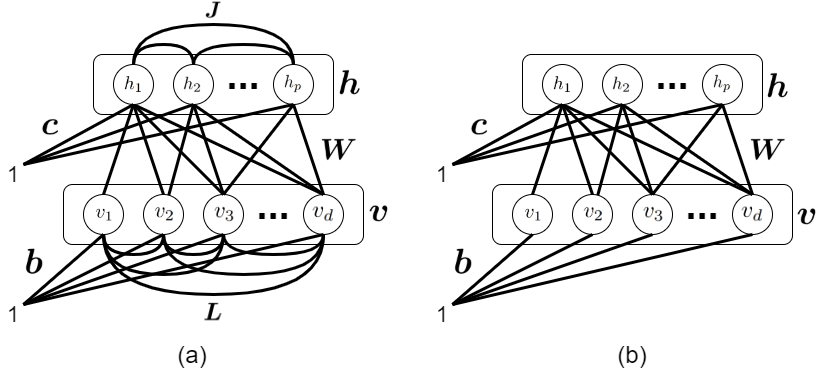
\includegraphics[width=\textwidth,height=\textheight,keepaspectratio]{img/rbm.png}
	\centering
	\caption{The structure of (a) a Boltzmann machine and (b) a restricted  Boltzmann machine \cite{Ghojogh.2021}}
	\label{fig:bm-rbm}
\end{figure}

\textit{Boltzmann machine (BM)} is a generative model and a
\textit{probabilistic graphical model (PGM)} \cite{Bishop.2006}. It consists of
a visible (or observation) layer
$\mathbf{v}=[v_1,v_2,\ldots,v_d]\in\mathbb{R}^d$ and a hidden layer of latent
variables $\mathbf{h}=[h_1,h_2,\ldots,h_p]\in\mathbb{R}^p$. The elements of both
layers contain binary values, i.e., $\forall i,j$, $v_i\in\{0,1\}$ and
$h_j\in\{0,1\}$. While the visible layer usually contains data (or other values
we can see), the hidden layer represents latent variables. In the PGM of BM,
there are connections between the elements $\mathbf{v}$ and $\mathbf{h}$ - both
within and between the layers. Each of the elements of both $\mathbf{v}$ and
$\mathbf{h}$ also has a bias. In a Restricted Boltzmann Machine (RBM), only
inter-layer links are allowed. Figure~\ref{fig:bm-rbm} depicts both of them with
their layers and links. Let $w_{ij}$ denote a link between $v_i$ and $h_j$,
$b_i$ be the bias link for $v_i$ and $c_j$ be the bias link for $h_i$. The whole
model can then be described in a matrix form: 
\begin{samepage}
	\begin{itemize}
		\item $\mathbf{W}=[w_{ij}]\in\mathbb{R}^{d\times p}$
		\item $\mathbf{b}=[b_1,b_2,\ldots,b_d]\in\mathbb{R}^d$
		\item $\mathbf{c}=[c_1,c_2,\ldots,c_p]\in\mathbb{R}^p$
	\end{itemize}
\end{samepage}
An RBM is what is called an Ising model \cite{Ising.1925}, thus having an
internal energy. According to \citet{Hinton.1983}, the energy of an RBM based on
interactions between linked units can be modelled as
\begin{equation}
	\mathbb{R}\ni E(\mathbf{v},\mathbf{h}):=-\mathbf{b}^T\mathbf{v}-\mathbf{c}^T\mathbf{h}-\mathbf{v}^T\mathbf{W}\mathbf{h}
	\label{eq:E_rbm}
\end{equation}
Training an RBM amounts to minimizing this energy. This brings the links and
biases of both layers to a state in which the hidden layer is capable of
capturing meaningful features or embeddings for the visible data. Two commonly  
used training algorithms for RBMs are \textit{Gibbs sampling} (Algorithm~
\ref{alg:gibbs-sampling}) and a \textit{constrastive divergence} 
(Algorithm~\ref{alg:contr-div}) which is based on it.

\begin{algorithm}
    \caption{Gibbs sampling in RBM}
    \label{alg:gibbs-sampling}
	\KwIn{visible dataset $\mathbf{v}$, (intialization: optional), number of steps $n$}
	Get initialization or do random initialization of $\mathbf{v}$\;
	\For{$i$ \KwFrom $1$ \KwTo $n$}{
		\For{$j$ \KwFrom $1$ \KwTo $p$}{
			$h_j^{(v)}\sim\mathbb{P}(h_j|\mathbf{v}^{(v)})$
		}
		\For{$i$ \KwFrom $1$ \KwTo $d$}{
			$v_i^{(v+1)}\sim\mathbb{P}(v_i|\mathbf{h}^{(v)})$
		}
	}
\end{algorithm}

\begin{algorithm}
	\caption {Training RBM using contrastive divergence}
	\label{alg:contr-div}
	\KwIn{training data $\{x_i\}_{i=1}^n$, number of Gibbs sampling steps $n$}
	Randomly initialize $\mathbf{W}$, $\mathbf{b}$, $\mathbf{c}$\;
	\KwWhile{not converged}{
		Sample a mini-batch
		$\{\mathbf{v}_1,\mathbf{v}_2,\ldots,\mathbf{v}_m\}$\; from training 
		dataset $\{\mathbf{x}_i\}_{i=1}^n$ (n.b. we may set $m=n$)\;
		\tcp{Gibbs sampling for each data point}
		Initialize $\hat{\mathbf{v}}_i^{(0)}\gets\mathbf{v}_i$ for all
		$i\in\{1,2,\ldots,m\}$\;
		\For{$i$ \KwFrom $1$ \KwTo $m$}{
			$\text{Algorithm~\ref{alg:gibbs-sampling}}\gets\hat{\mathbf{v}}_i^{(0)}$\;
			$\{h_i\}_{i=1}^p,\{v_i\}_{i=1^d}\gets$ Last iteration of 
			Algorithm~\ref{alg:gibbs-sampling}\;
			$\tilde{\mathbf{h}}_i\gets[h_1,h_2,\ldots,h_p]^T$\;
			$\tilde{\mathbf{v}}_i\gets[v_1,v_2,\ldots,v_d]^T$\;
			$\hat{\mathbf{h}}_i\gets\mathbb{E}_{\sim\mathbb{P}(\mathbf{h}|\mathbf{v}_i)}[\mathbf{h}]$\;
		}
		\tcp{gradients:}
		$\nabla_\mathbf{W}\ell(\theta)\gets\sum_{i=1}^m\mathbf{v}_i\hat{\mathbf{h}}_i^T-\sum_{i=1}^m\tilde{\mathbf{h}}_i\tilde{\mathbf{v}}_i^T$\;
		$\nabla_\mathbf{b}\ell(\theta)\gets\sum_{i=1}^m\mathbf{v}_i-\sum_{i=1}^m\tilde{\mathbf{v}}_i$\;
		$\nabla_\mathbf{c}\ell(\theta)\gets\sum_{i=1}^m\mathbf{h}_i-\sum_{i=1}^m\tilde{\mathbf{h}}_i$\;
		\tcp{gradient descent for updating solution:}
		$\mathbf{W}\gets\mathbf{W}-\nu\nabla_\mathbf{W}\ell(\theta)$\;
		$\mathbf{b}\gets\mathbf{b}-\nu\nabla_\mathbf{b}\ell(\theta)$\;
		$\mathbf{c}\gets\mathbf{c}-\nu\nabla_\mathbf{c}\ell(\theta)$\;
	}
\end{algorithm}

\clearpage

\subsection{Stacking RBM models}
\begin{figure}
	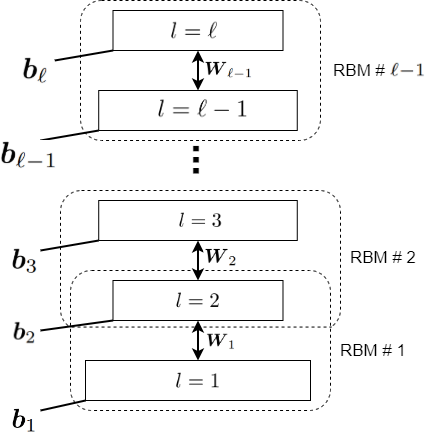
\includegraphics[height=0.4\textwidth,keepaspectratio]{img/dbn.png}
	\centering
	\caption{Pre-training a deep belief network by considering every pair of layers as an RBM \cite{Ghojogh.2021}}.
	\label{fig:dbn}
\end{figure}
A DBN consists of several RBM models stacked together, as depicted on
Figure~\ref{fig:dbn}. The first layer of the model accepts the input data as
it's visible layer $\mathbf{v}_1$. Then, on each layer $\ell$, an RBM model with
the visible layer $\mathbf{v}_\ell$ has the hidden layer $\mathbf{h}_\ell$ that
is acts as the visible layer $\mathbf{v}_{\ell+1}$ for the RBM above it.
Training a DBN is described in Algorithm~\ref{alg:train-dbn} and supposes
optimizing all RBM components layer by layer via Algorithm~\ref{alg:contr-div}
followed by error backpropagation.

\begin{algorithm}[b!]
	\caption {Training a deep belief network}
	\KwIn{training data $\{\mathbf{x}_i\}_{i=1}^n$}
	\For{$l$ \KwFrom $1$ \KwTo $\ell-1$}{
		\eIf{$l=1$}{
			$\{\mathbf{v}_i\}_{i=1}^n\gets\{\mathbf{x}_i\}_{i=1}^n$\;
		}{
			\tcp{generate $n$ hidden variables of previous RBM:}
			$\{\mathbf{h}_i\}_{i=1}^n\gets$ Algorithm~\ref{alg:gibbs-sampling}
			for $(l-1)$-th RBM$\gets\{\mathbf{v}_i\}_{i=1}^n$\;
			$\{\mathbf{v}_i\}_{i=1}^n\gets\{\mathbf{h}_i\}_{i=1}^n$
		}
		$\mathbf{W}_l,\mathbf{b}_l,\mathbf{b}_{l+1}\gets$
		Algorithm~\ref{alg:contr-div} for $l$-th RBM
		$\gets\{\mathbf{v}\}_{i=1}^n$
	}
	\tcp{fine-tuning using backpropagation:}
	Initialize network with weights $\{\mathbf{W}_l\}_{l=1}^{\ell-1}$
	and biases $\{\mathbf{b}_l\}_{l=2}^n$\;
	$\{\mathbf{W}_l\}_{l=1}^{\ell-1},\{\mathbf{b}_l\}_{l=1}^\ell\gets$
	Backpropagate the error of loss from several epochs
	\label{alg:train-dbn}
\end{algorithm}

\section{Kernel extreme learning machine}

The kernel extreme learning machine is known to be dealing well with
non-linear time series, which justifies it's use for traffic flow data.

\textit{Extreme learning machines (ELM)} are feedforward neural networks whose
input weights $\mathbf{W}_{in}$ and biases $\mathbf{b}_in$ for the hidden nodes
are assigned randomly and fixed rather than being optimized iteratively (via
gradient descent, annealing etc.). The output of each hidden node for the input
$\mathbf{X}$ then becomes
\begin{equation}
	\mathbf{H}=h(X)=f(\mathbf{X}\cdot\mathbf{W}_in+\mathbf{b}_in)
	\label{eq:H}
\end{equation}
for the actifation function $f$. The output for the whole network is
\begin{equation}
	\mathbf{Y}=\mathbf{H}\cdot\mathbf{W}_{out}.
	\label{eq:Y_elm}
\end{equation}
The correct prediction is achieved via calculating the optimal output weights
$W_{out}$ analytically in one step (again, without gradual optimization):
\begin{equation}
	\mathbf{W}_{out}=
	\mathbf{H}^\dagger=(\mathbf{H}^T\cdot\mathbf{H})^{-1}\cdot T
	\label{eq:W_out}
\end{equation}
for the target values $T$.

\textit{Kernel} extreme learning machines replace the random mapping of
ELM with kernel mapping. Define the kernel learning mapping as
\begin{equation}
	\mathbf{\Omega}_{ELM}=\mathbf{H}\mathbf{H}^T.
	\label{eq:Omega}
\end{equation}
Since $H$ is obtained by applying weights, biases and activation to the input,
and it's outer product with itself is taken as the final result, we can replace 
the whole operiation with a kernel function $k$:
\begin{equation}
	\mathbf{\Omega}_{ELM}=h(x_i)h(x_j)=k(x_i,x_j).
\end{equation}
Specifically, \citet{Han.2020} use a Gaussian kernel function here:
\begin{equation}
	k(x,x_j)=\exp(-\gamma\cdot||x-x_i||^2),\gamma>0.
	\label{eq:Gaussian_kernel}
\end{equation}
Regularization using a coefficient $C$, inversion and multiplication with the
target values produces the relation matrix $\mathbf{\beta}$:
\begin{equation}
	\mathbf{\beta}=(\frac{I}{C}+\mathbf{\Omega}_{ELM})^{-1}T.
	\label{eq:beta}
\end{equation}
This is then used with the kernel multiplication of each new unit and the
original training data to predict the output for an unsees input $x$:
\begin{equation}
	\begin{split}
		f(x)=[k(x,x_1),k(x,x_2),\ldots,k(x,x_N)]\mathbf{\beta} \\
		=[k(x,x_1),k(x,x_2),\ldots,k(x,x_N)]
		(\frac{I}{C}+\mathbf{\Omega}_{ELM})^{-1}T.
	\end{split}
	\label{eq:kelm-inference}
\end{equation}


\section{Complete prediction procedure}

The DBN-KELM model is composed of DBN which is respondible for feature
extraction and KELM for prediction. The architecture as depicted on
Figure~\ref{fig:dbn-kelm} consists of four hidden layers - three RBMs forming a
DBN model and a single hidden layer of a kernel extreme learning machine. In
other words, the output of DBN is embedded features that are then fed to the
KELM model.

The DBN part of the model is trained using the \textit{mean square error (MSE)} 
loss:
\begin{equation}
	MSE=\frac{1}{N}\sqrt{\sum_{i=1}^N(y_i-\hat{y}_i)}.
	\label{eq:mse}
\end{equation}
This loss function is also used for the final evaulation of the direct
prediction (applying DBN+KELM to the columns of $\mathbf{C}$). The prediction
after reconstruction via Equation~\ref{eq:Q} (for sections not participating in
direct prediction) a \textit{mean absolute percentage error (MAPE)} function is
used:
\begin{equation}
	MAPE=\frac{1}{N}\sum_{i=1}^N\bigg |\frac{(y_i-\hat{y}_i)}{y_i}\bigg |
	\times 100\%
	\label{eq:mape}
\end{equation}

\begin{figure}
	\centering
	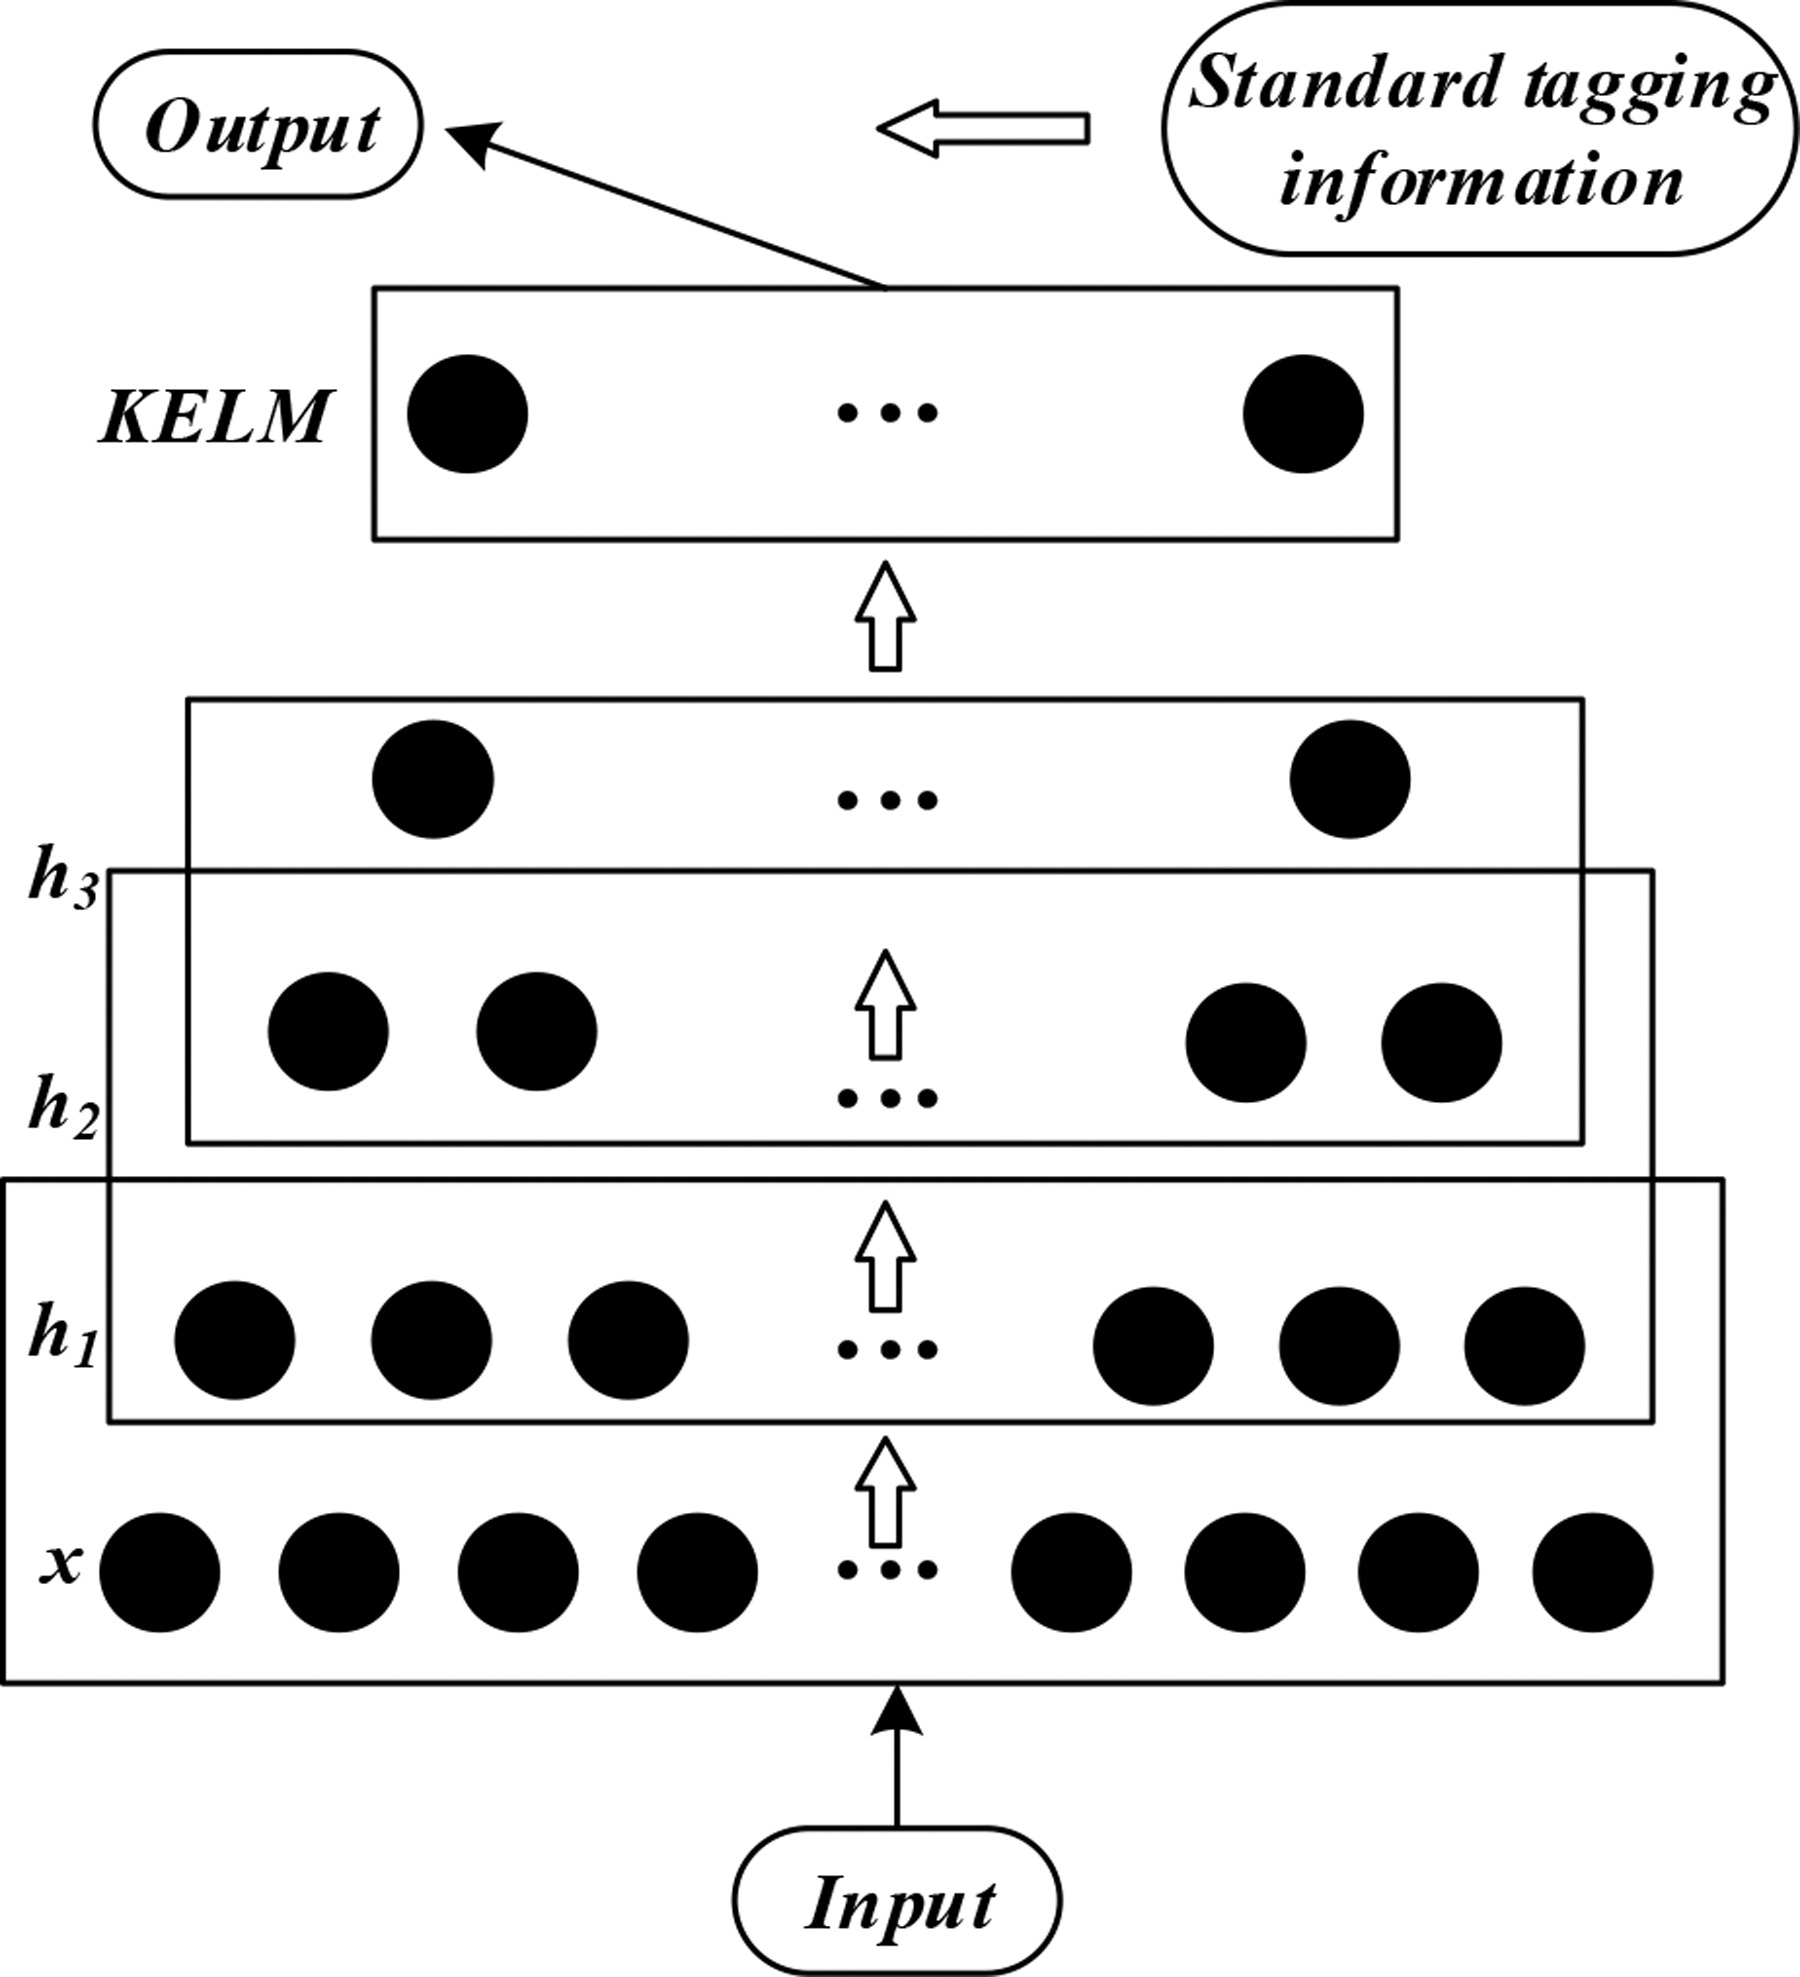
\includegraphics[height=0.3\textheight,keepaspectratio]{img/dbn-kelm.jpg}
	\caption{Structure of DBN-KELM \cite{Han.2020}}
	\label{fig:dbn-kelm}
\end{figure}
\begin{figure}
	\centering
	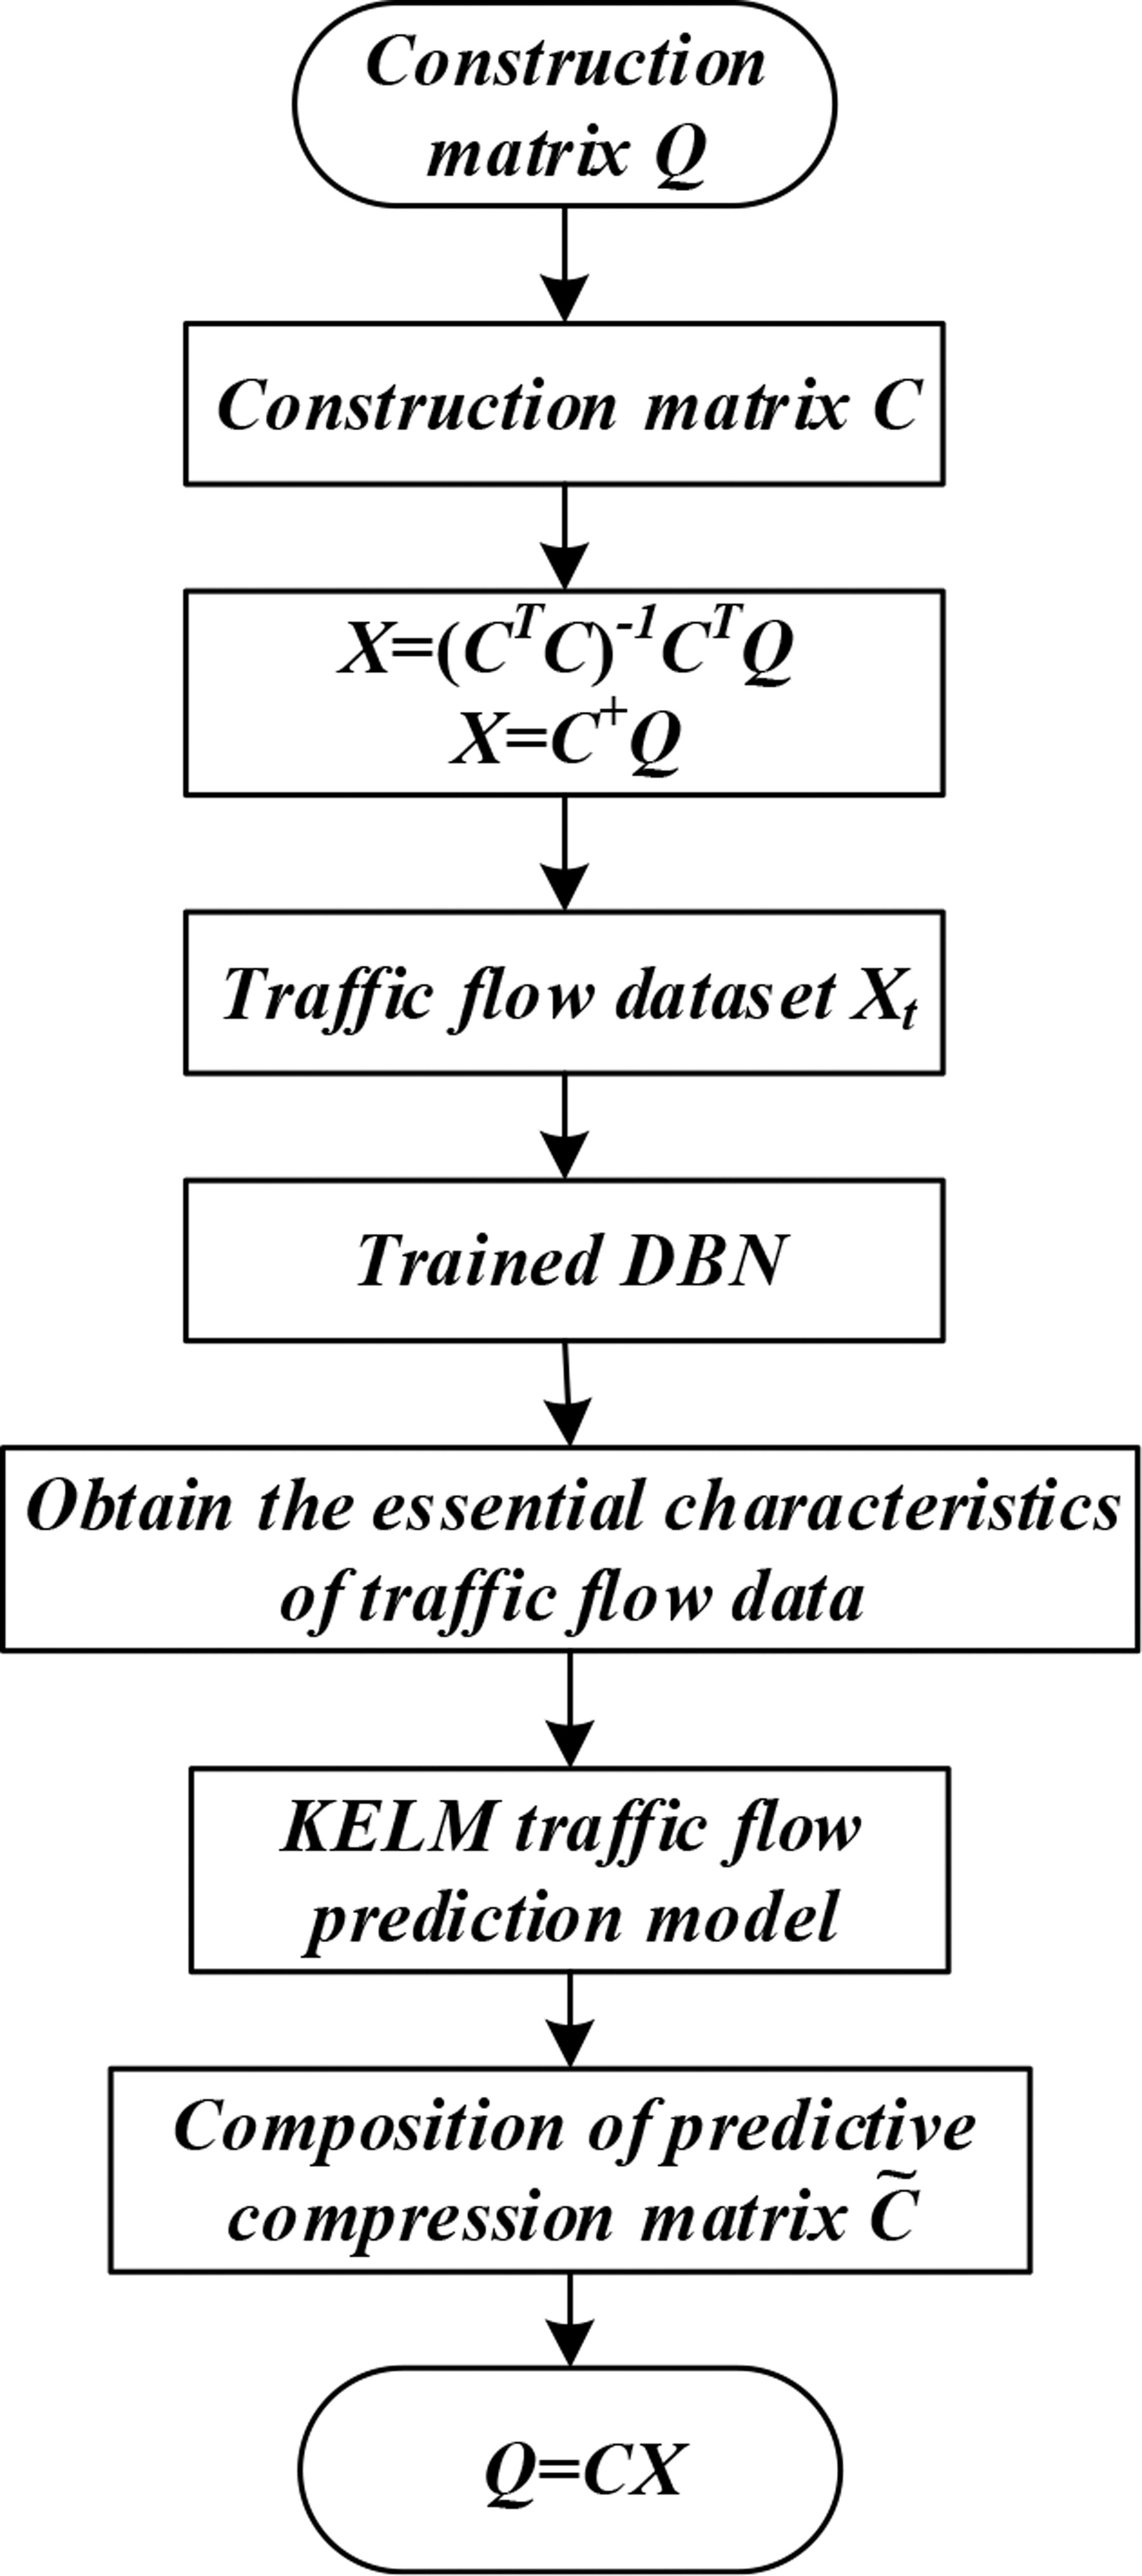
\includegraphics[height=0.3\textheight,keepaspectratio]{img/steps.jpg}
	\caption{Processing steps of the whole prediction model \cite{Han.2020}}
	\label{fig:steps}
\end{figure}

\begin{samepage}
	The prediction procedure is depicted in Figure~\ref{fig:steps}:
	\begin{itemize}
		\item[\textit{Step 1:}] Construct the road network data matrix
		$\mathbf{Q}$
		from the raw input data.
		\item[\textit{Step 2:}] Use the compression method to find a
		CX-decomposition of $\mathbf{Q}$. Select a subset of the data - the
		compression matrix $\mathbf{C}$, as well as the relation matrix
		$\mathbf{X}$
		(see Equation~\ref{eq:X})
		to extend the prediction to the whole network in the future.
		\item[\textit{Step 3:}] Preprocess the data from $\mathbf{C}$ by
		splitting
		it into the \textit{trend} and the \textit{residual} components via
		Fourier
		transform (see Section~\ref{sec:extraction-of-components}).
		\item[\textit{Step 4:}] Predict:
		\begin{itemize}
			\item the next sample in the trend term with the (Overlap-)SSA
			method;
			\item the next sample in the residuel term with a previously trained
			combined DBN-KELM model.
		\end{itemize}
		\item[\textit{Step 5:}] Form the predicted compression matrix
		$\tilde{\mathbf{C}}$ by adding back the trend and residual terms after
		prediction - Equation~\ref{eq:X_tilde}.
		\item[\textit{Step 6:}] Obtain the prediction $\tilde{\mathbf{Q}}$ for
		the whole network by applying Equation~\ref{eq:Q} to
		$\tilde{\mathbf{C}}$ and the previously calculated relation matrix
		$\mathbf{X}$:
		\begin{equation}
			\tilde{\mathbf{Q}}=\tilde{\mathbf{C}}\mathbf{X}
			\label{eq:Q_tilde}
		\end{equation}
	\end{itemize}
\end{samepage}


\chapter{Implementation}

\section{Data preparation and rectifying} \label{sec:data-preparation}

On top of processing and merging some parts of the data to adapt it for the
needs of the described method (see Section~\ref{sec:expected-data}), analysis 
has revealed missing points and mistakes in the provided files, that needed to 
be solved first. For convenience, we wrote a Python script capable of resolving
all these issues automatically given the original corrupt files.

\begin{enumerate}
	\item Some entries in the \textit{Look Up Table} contained spelling
	mistakes, i.e., extra or missing brackets, whitespaces, incorrect indices in
	detector names etc.
	\item For some intersections, namely \textit{2040}, \textit{4170} and 
	\textit{8007}, the detector data are missing entirely, i.e.,
	the tables are defined in corresponding csv-files, but are completely empty.
	Unfortunately, there were no alternative sources known for these data.
	Therefore, these intersections were ignored in further experiments.
	\item Some files, for example, \textit{DetCount\char`_20210721.csv} for the 
	intersection.
	\textit{6010}, are missing the csv header. Assuming that the order of 
	columns has to be the same for all files in the same folder, we
	copied the headers from files. This assumption was justified by the fact
	that this order was the same for all files having the header, and was
	alphabetical with regards to corresponding detector names.
	\item Others, like \textit{DetCount\char`_20210429.csv} for the intersection
	\textit{8403}, had only the \textit{DATUM} column in them, with the names of
	detectors missing. Solved the same way as the completely missing headers
	by copying from other files in the folder.
	\item This solution, however, would not work for the intersection
	\textit{3050}, since none of it's files contained the header. We had to
	reconstruct it manually and insert it into one of the files before letting
	our script copy it to the other tables in the same folder.
	\item Some files, e.g., \textit{DetCount\char`_20211215.csv} for
	\textit{8403}, are missing values in several first rows. Our script fills
	them with zeros.
	\item For intersection \textit{6021}, there are files with two types of
	headers. Some, like \textit{DetCount\char`_20210101.csv}, contain columns
	for 9 detectors, while others, for example,
	\textit{DetCount\char`_20210416.csv} - for 11. For the first type of files,
	we inserted the missing 2 columns and filled them with zeros.
	\item In all folders, the file \textit{DetCount\char`_20211031.csv} gives
	two conflicting readings on four time stamps from \textit{02:00:00} to
	\textit{02:45:00}. It is unclear what the problem has come from and which
	version is correct (since they are different), but we have decided to remove
	the first copy of these time stamps and keep the second one in each file.
	\item Some 4-digit codes actually denoted groups of, rather than separate
	intersections. However, this was not reflected in the folder structure of
	the data set. Therefore, our script had to split the tables by extracting
	the detector columns from all csv-files and grouping them according the the
	real separation of these groups (as derived from the Look Up Table). These
	intersections and their splittings include:
	\begin{itemize}
		\item \textit{3060} - into \textit{3060}, \textit{3060\char`_G} and 
		\textit{3060\char`_L};
		\item \textit{5090} - into \textit{5090\char`_Teilknoten 1} and
		\textit{5090\char`_Teilknoten 2};
		\item \textit{6010} - into \textit{6010\char`_F1a} and
		\textit{6010\char`_F1b}.
	\end{itemize}
\end{enumerate}


\section{Code structure and design} \label{sec:impl-details}

An official implementation for the approach authored by \citet{Han.2020} and
described above is not provided online. For this project, we have resorted to
implementing all methods by hand as much as the overview in the paper has
allowed. Our code is written in \textit{Python} using the \textit{PyTorch}
module for both data processing and model training. All essential steps were
first realised and tested as separate \textit{Jupyter Notebooks} - and then put
together into a single module for running the complete procedure. This section 
provides details on how each portion of the method was implemented.


\subsection{Procedure steps}

This section explains how we have implemented all basic steps of the described
procedure. The logic for all these steps is extracted to separate modules with
step-related Jupyter notebooks merely calling their procedures for debugging.
The last step uses all those modules combined to execute the whole method.

\textbf{Step 1. Data extraction.} As described in Section~\ref{sec:data-preparation}, our data provide the values
separately for each detector on the entrance to the intersection. The expected 
traffic flow matrix $\mathbf{Q}$, on the other hand, has counts for each section
combined, where the section is a connection between two intersections in one
direction (see Section~\ref{sec:expected-data}). Therefore, our first goal was
to aggregate the lanes on each intersection by their sources and sum the values
from their corresponding detectos. The information for this aggregation can be
obtained from the provided Look Up Table.

\textbf{Step 2. Data compression.} As described in
Section~\ref{sec:data-grouping-and-compression}, the basis for the data
compression step is computing the Pearson correlation coefficient via 
Equation~\ref{eq:R_i_j} and building a matrix $R$ from the computed values.
PyTorch already provides an implementation for these two step in a one 
convenient function \texttt{torch.corrcoeff}. Whether the data are still corrupt
or some sections of the network were completely unused in the analysed time
period, but the input matrix $\mathbf{Q}$ contains columns filled entirely with
zeros. This results in zero-division, breaking the computation of correlation
coefficients. To tackle the issue, we exclude the zero-sequences on this step
and work only with the remaining part of $\mathbf{Q}$. The rest of the steps is
implemented more or less as supposed in the original paper, with the
representative of each section group being selected as the first one indexed.

\textbf{Step 3. Data preprocessing.} The traditional way of using the discrete
form of the Fourier tranform is \textit{Fast Fourier Transform (FFT)}. PyTorch
includes an implementation of this algortihm available as
\texttt{torch.fft.fft}. Another function called \texttt{torch.fft.ifft}
performes the inverse operation, i.e., converts a frequency-domain signal to a
time-domain. Since the output of FFT is in complex numbers, we have to take
their real part for further processing.

\textbf{Step 4. Model training.} The training process was not described in the
paper explicitly, but could be derived from the models descriptions.

Before training and validating our methods on data, we have to normalize them to
a fixed range. Since the sections vary a lot in their traffic activity, we deal
with very different ranges in their raw forms. Therefore, we first find the
largest value in each series to divide all entries by them and store them
separately to multiply the predictions back after forecasting. This way, during
the prediction process our methods have to only deal with values between $0$ and
$1$. We can then turn to realizing the training procedure itself.

First of all, the adopted description of RBMs states that each node contains a
binary value. This contradicts the fact that our data are given as integers of
arbitrary size (or floating-point numbers after normalization). This discrepancy
is never addressed in the original paper. Since pre-training via RBM
optimization plays the same role as initialization in a traditional deep neural
network, we assumed that the binary values used for RBM optimization are not
related to the data used in the end, and performed this step with randomly
initialized binary vectors.

Apart from that, it is mentioned in Algorithm~\ref{alg:train-dbn} that the
training procedure for DBN requires multiple refinement steps of gradient
descent. KELM, on the other hand, is fitted in one single operation. At the same
time, KELM expects features correctly extracted by a trained DBN, while DBN is
trained using a loss function of an output of KELM. We need to propagate the DBN
loss on each training step through a KELM which is trained instantly. The only
consistent way to do so is to re-fit KELM after each iteration. Thus, our 
procedure looks like this:
\begin{enumerate}
	\item Pre-train DBN as described in lines 1-10 of Algorithm~\ref{alg:train-dbn}.
	\item Use the DBN to extract features from the training data.
	\item Fit KELM to predict the next-step value from the extracted features.
	\item Use the combined DBN+KELM model again to make predictions.
	\item Calculate the loss using MSE (Equation~\ref{eq:mse}), propagate it
	through the unified model and update DBN.
	\item Repeat all the steps from 2 for the chosen number of training epochs.
\end{enumerate}
This way, we iterate between updating weights of DBN using an "old" KELM and
fitting a "new" KELM for working with an updated DBN.

MSE (Equation~\ref{eq:mse}) used for model training and per-section evaulation,
as well as MAPE (Equation~\ref{eq:mape}) for evaluation after reconstruction
(via Equation~\ref{eq:Q_tilde}) are both available in the \texttt{torchmetrics}
module as \texttt{MeanSquaredError} and \texttt{MeanAbsolutePercentageError}
respectively.

\citet{Han.2020} do not specify explicitly whether the same trained instance
DBN-KELM is to be shared for all sections or a new one created for each of them.
We have decided to try both approaches.

Finally, in the original paper, the authors highlight a difference in
periodicity of the traffic flow on week days versus week ends. Hence, they
consider both of them separately, making it necessary to create a data set that
would consider only one type of days. We split the complete input matrix
$\mathbf{Q}$ using a utility function that counts samples per day and uses the
\texttt{datetime} library to separate the dates. Our final data class derived
from \texttt{torch.utils.data.Dataset} uses a sliding window returning it's
contents as an input and the next sample after it as the expected output. During
this sliding process, it also makes sure to not divide the window between
consecutive regions (e.g., start on Sunday and end on Saturday of the next
week).

\subsection{Prediction methods}

Here we give brief details of our implementation for the prediction methods.

\textbf{Restricted Boltzmann machine.} For the RBM class, as well as the
training algortihm, there is an available open-source algorithm
\cite{Nguyen.2019}. The only change we had to do to their code was extracting
forward propagation step (the affine linear layers with \texttt{torch.sigmoid}
activation) into a separate function. This was necessary as the original was
intended as a standalone model, rather than a component for a larged DBN
architecture.

\textbf{Deep Belief Network.} Since the DBN was to be fine-tuned using gradient
descent, it was worth declaring it as a child class of \texttt{torch.nn.Module}
with an override for the \texttt{forward} method using the forward propagation
method added for the RBMs. The RBMs themselves are stored in a member
\texttt{torch.nn.ModuleList}, which is a standard for implementing deep models
in PyTorch.

\textbf{Kernel extreme learning machine}. Equation~\ref{eq:kelm-inference} shows
that inputs $x$ from the original training data for KELM have to be passed to
the kernel function during inference on new inputs. Thus, they have to be stored
as a class member when fitting the model. The same is true for the matrix
$\mathbf{\beta}$ which depends on the training ground truth. Gradient descent
would not be used in this model, but it would for fine-tuning of the DBN. And
since KELM is to be attached directly to the DBN, both $x$ and $\mathbf{\beta}$
have to support the gradient propagation performed by PyTorch's autograd. For
this reason, we store them as instances of the \texttt{torch.nn.Parameter}
class.

\textbf{Singular spectrum analysis}. Implementing the SSA, we closely followed
\citet{Golyandina.2014}. Before the forecasting method, we tested the whole
approach by using it for decomposition to check if adding extracted components
back together yields the original signal. Since the hyper parameters $I$ and $L$
are shared between both applications of the method, it made sense to implement
it as a whole new class, rather than a function, and store the $I$ and $L$ as
it's members. On top of that, for successful forecasting we need to use the
reconstraction as an intermediate step, while keeping an access to the
eigentriples calculated in the process. For this purpose, we split the
deconstruction into embedding, singular value decomposition and sequences
generation implemented as three different methods of the class. On a lower
level, like for the other methods, all matrix operations are done using PyTorch.


\chapter{Experiments and results}

\section{Data analysis}

Planning our experiments started with analysis of the data at hand.
\citet{Han.2020} treat week days and week ends separately. The motivation behind
this is the difference in periodicity. With data collected by the American
Traffic Research Data Laboratory, each week they observe two peaks in traffic
flow every day from Monday to Friday and only one on Saturday and Sunday. This
does not correspond exactly to what we can see on the data from Ingolstadt. Or
at the very least, not for all weeks and sections, as illustrated on
Figure~\ref{fig:week-data}. Nevertheless, it is possible to see  differences in
data behaviour with an inclination towards what is indicated in the original
work. While we cannot see clear peaks during week days, the most of activity is
still spread more widely through the day. On week ends, however, the peak hours
are concentrated in a narrower point with less traffic flow around it. We
conclude that splitting data into week ends and week days is similarly justified
in our case.

\begin{figure}
	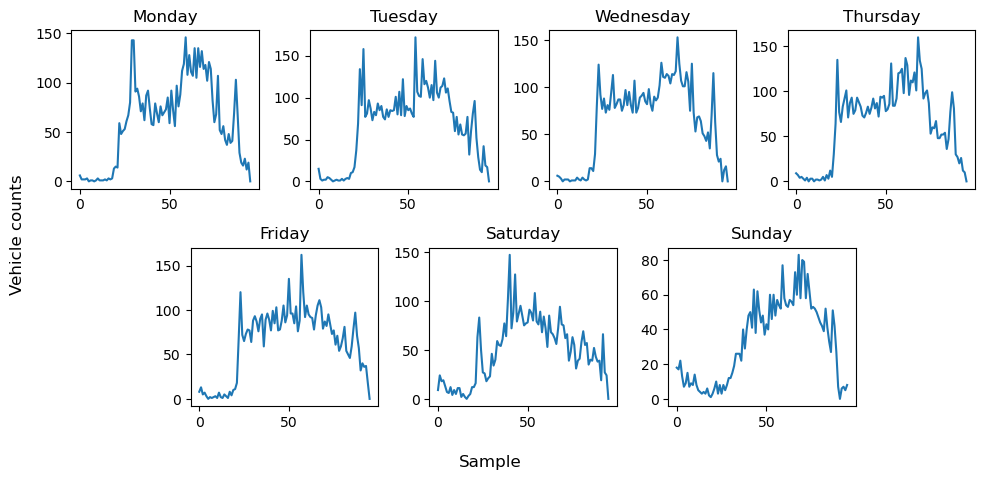
\includegraphics[width=\textwidth,keepaspectratio]{img/week_data.png}
	\centering
	\caption{Traffic flow in vehicle counts per 15-minute sample taken on one section from the Ingolstadt road network during a week from \textit{June 7} to \textit{June 13, 2021}.}
	\label{fig:week-data}
\end{figure}

The next step in our analysis is checking the degree of correlation between
sections of the network. This aspect of the data is relevant for the compression
step described in Section~\ref{sec:data-grouping-and-compression}. The outcome
of that step is dependent on our choice of the $\alpha$ hyper parameter.
Specifically, two sections are inserted into one group if their correlation
coefficient exceeds the pre-defined $\alpha$ (i.e., $R(i,j)>\alpha$, as defined
in Equation~\ref{eq:R_i_j}) or different ones otherwise. Therefore, raising the
value of $\alpha$ decreases the probability of placing two sections into one
group, thus potentially increasing the number of groups in the end. The exact
dependency between the value of $\alpha$ and the resultant number of groups in
our data specifically is given in Figure~\ref{fig:alpha-groups}.

\begin{figure}
	\centering
	\begin{minipage}{0.45\textwidth}
		\centering
		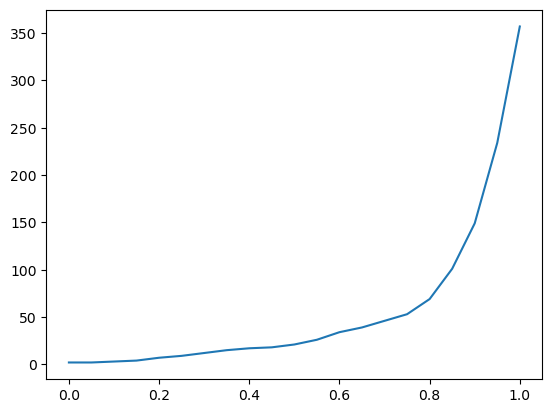
\includegraphics[width=\textwidth,height=\textheight,keepaspectratio]{img/alpha_groups_0.5_0.95.png}
		\subcaption{$\alpha\in[0.05,0.95]$}
	\end{minipage}
	\begin{minipage}{0.45\textwidth}
		\centering
		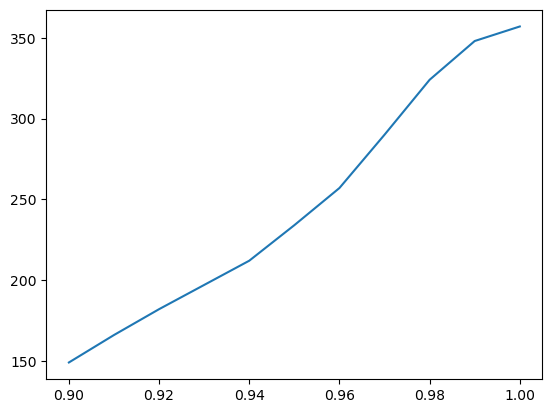
\includegraphics[width=\textwidth,height=\textheight,keepaspectratio]{img/alpha_groups_9.0_9.9.png}
		\subcaption{$\alpha\in[0.9,0.99]$}
	\end{minipage}
	\begin{minipage}{\textwidth}
		\centering
		\begin{tabular}{c|c|c|c|c|c|c|c|c|c|c}
			$\mathbf{\alpha}$ & $0.90$ & $0.91$ & $0.92$ & $0.93$ & $0.94$ &
			$0.95$ & $0.96$ & $0.97$ & $0.98$ & $0.99$ \\
			\hline
			\textbf{Number of groups} & $149$ & $166$ & $182$ & $197$ & $212$ &
			$234$ & $257$ & $290$ & $324$ & $348$
		\end{tabular}\\
		\begin{tabular}{c|c|c|c|c|c|c|c|c|c|c}
			$\mathbf{\alpha}$ & $0.05$ & $0.15$ & $0.25$ & $0.35$ & $0.45$ &
			$0.55$ & $0.65$ & $0.75$ & $0.85$ & $0.95$ \\
			\hline
			\textbf{Number of groups} & $2$ & $4$ & $9$ & $15$ & $18$ & $26$ &
			$39$ & $53$ & $101$ & $234$
		\end{tabular}
	\end{minipage}
	\caption{The number of groups formed from the sections in available data depending on the selected value of the hyper parameter $\alpha$.}
	\label{fig:alpha-groups}
\end{figure}


\section{Outline}

For training and evaluation of the methods, we select four whole consecutive
weeks from \textit{May 31 to June 27, 2021} for the final prediction. Since the
prediction process is split into two independent parts as described in
Section~\ref{sec:extraction-of-components}, our plan is to choose three  sets of
best hyper parameters: minimizing the loss for trend, for the residuals
and for the combined predicted signal.

The input window for each call to the model was 1 hour long in the original
paper. For 5-minute sampling intervals, that amounts to 12 samples. However,
since in our data the readings are sampled only every 15 minutes, that would
produce 4 samples as the input. Thus, we have chosen to use a 3-hour window to
keep the number of samples at 12. This sliding procedure generates a sequence of
12-sample vectors and single-sample ground truths. We divide this sequence in a
80\%/20\% ratio to leave a part of data for validation. We use the resultant
data set for training and validating DBN-KELM.

For trend prediction, it is not enough to use a 12-sample window. Since SSA is a
non-parametric method, it's forecasting ability depends solely on data
periodicity, which can be captured from a longer sequence only. Therefore, we
extend the input window by shifting it's starting point to the beginning of the
year. This approach could prove useful for the residual prediction as well,
since it would give the model more data to train on. However, this would
result in an excessive memory usage making it infeasible to fit KELM to the
whole data. Therefore, we stick with applying both methods to different input
periods ending at the same time point.

In the first session of runs, we determine the optimal values for the hyper
parameters. There are three that we are interested in:
\begin{itemize}
	\item spectral threshold $P$ for splitting the series into two components as
	described in \textit{Step 2} in the end of
	Section~\ref{sec:extraction-of-components};
	\item output number of hidden nodes $N$ of DBN, i.e., the dimensionality of
	extracted features to be passed to KELM;
	\item threshold $\alpha$ on correlation coefficient that defines the group
	splitting during the compression procedure (\textit{Step 3} in the end of
	Section~\ref{sec:data-grouping-and-compression}).
\end{itemize}
The first two parameters define per-section prediction, while the third is used
only when utilizing the compression. Therefore, we adjust the parameters in two
stages, using MSE loss to adjust $P$ and $N$ and MAPE for optimizing over
$\alpha$ (Equations \ref{eq:mse} and \ref{eq:mape} respectively).

After that, we apply the procedure to all sections and report our results using
the same losses.


\section{Method and parameters adjustment}

Test runs of our method have proven infeasible to train one shared DBN-KELM on
all sections data. Even if the model architecture is flexible enough to capture
all intricacies in predicting the residuals, the memory requirements in that
case could not be satisfied. This is due to the fact that fitting a KELM model
requires storing the original data as a class member for further inference (see
Equation~\ref{eq:kelm-inference}). For 3-hour sliding windows shifted by 15
minutes each, this means $(24-3)*15=315$ input sequences per section per day.
Storing them in an optimized form is not possible either since they are needed
in calculation of $\beta$ which is also stored. After unsuccessful attempts to
run this configuration in various advanced machines, including the one with a
\textit{T4} GPU with \textit{16 GB GPU RAM} available in \textit{Google Colab},
we have resorted to training a separate model for each section. An alternative
would be to train a model on a limited amount of data and still generalize it to
all sections at once. This could be done by either training it on only one
section, on just a handful of samples from multiple sections. Both approaches,
however, are reasonable only under an assumption that the traffic flow is indeed
uniform across all of them and the per-section prediction accuracy of our model
is very high.

For the initial runs, we apply our method to six sections as a sanity check and
select one of them with more active traffic flow to optimize the hyper
parameters.

\chapter{Discussion}


%\todo{If you want to remember a task, place it here.}
